% Options for packages loaded elsewhere
\PassOptionsToPackage{unicode}{hyperref}
\PassOptionsToPackage{hyphens}{url}
\documentclass[
]{article}
\usepackage{xcolor}
\usepackage[margin=1in]{geometry}
\usepackage{amsmath,amssymb}
\setcounter{secnumdepth}{-\maxdimen} % remove section numbering
\usepackage{iftex}
\ifPDFTeX
  \usepackage[T1]{fontenc}
  \usepackage[utf8]{inputenc}
  \usepackage{textcomp} % provide euro and other symbols
\else % if luatex or xetex
  \usepackage{unicode-math} % this also loads fontspec
  \defaultfontfeatures{Scale=MatchLowercase}
  \defaultfontfeatures[\rmfamily]{Ligatures=TeX,Scale=1}
\fi
\usepackage{lmodern}
\ifPDFTeX\else
  % xetex/luatex font selection
\fi
% Use upquote if available, for straight quotes in verbatim environments
\IfFileExists{upquote.sty}{\usepackage{upquote}}{}
\IfFileExists{microtype.sty}{% use microtype if available
  \usepackage[]{microtype}
  \UseMicrotypeSet[protrusion]{basicmath} % disable protrusion for tt fonts
}{}
\makeatletter
\@ifundefined{KOMAClassName}{% if non-KOMA class
  \IfFileExists{parskip.sty}{%
    \usepackage{parskip}
  }{% else
    \setlength{\parindent}{0pt}
    \setlength{\parskip}{6pt plus 2pt minus 1pt}}
}{% if KOMA class
  \KOMAoptions{parskip=half}}
\makeatother
\usepackage{color}
\usepackage{fancyvrb}
\newcommand{\VerbBar}{|}
\newcommand{\VERB}{\Verb[commandchars=\\\{\}]}
\DefineVerbatimEnvironment{Highlighting}{Verbatim}{commandchars=\\\{\}}
% Add ',fontsize=\small' for more characters per line
\usepackage{framed}
\definecolor{shadecolor}{RGB}{248,248,248}
\newenvironment{Shaded}{\begin{snugshade}}{\end{snugshade}}
\newcommand{\AlertTok}[1]{\textcolor[rgb]{0.94,0.16,0.16}{#1}}
\newcommand{\AnnotationTok}[1]{\textcolor[rgb]{0.56,0.35,0.01}{\textbf{\textit{#1}}}}
\newcommand{\AttributeTok}[1]{\textcolor[rgb]{0.13,0.29,0.53}{#1}}
\newcommand{\BaseNTok}[1]{\textcolor[rgb]{0.00,0.00,0.81}{#1}}
\newcommand{\BuiltInTok}[1]{#1}
\newcommand{\CharTok}[1]{\textcolor[rgb]{0.31,0.60,0.02}{#1}}
\newcommand{\CommentTok}[1]{\textcolor[rgb]{0.56,0.35,0.01}{\textit{#1}}}
\newcommand{\CommentVarTok}[1]{\textcolor[rgb]{0.56,0.35,0.01}{\textbf{\textit{#1}}}}
\newcommand{\ConstantTok}[1]{\textcolor[rgb]{0.56,0.35,0.01}{#1}}
\newcommand{\ControlFlowTok}[1]{\textcolor[rgb]{0.13,0.29,0.53}{\textbf{#1}}}
\newcommand{\DataTypeTok}[1]{\textcolor[rgb]{0.13,0.29,0.53}{#1}}
\newcommand{\DecValTok}[1]{\textcolor[rgb]{0.00,0.00,0.81}{#1}}
\newcommand{\DocumentationTok}[1]{\textcolor[rgb]{0.56,0.35,0.01}{\textbf{\textit{#1}}}}
\newcommand{\ErrorTok}[1]{\textcolor[rgb]{0.64,0.00,0.00}{\textbf{#1}}}
\newcommand{\ExtensionTok}[1]{#1}
\newcommand{\FloatTok}[1]{\textcolor[rgb]{0.00,0.00,0.81}{#1}}
\newcommand{\FunctionTok}[1]{\textcolor[rgb]{0.13,0.29,0.53}{\textbf{#1}}}
\newcommand{\ImportTok}[1]{#1}
\newcommand{\InformationTok}[1]{\textcolor[rgb]{0.56,0.35,0.01}{\textbf{\textit{#1}}}}
\newcommand{\KeywordTok}[1]{\textcolor[rgb]{0.13,0.29,0.53}{\textbf{#1}}}
\newcommand{\NormalTok}[1]{#1}
\newcommand{\OperatorTok}[1]{\textcolor[rgb]{0.81,0.36,0.00}{\textbf{#1}}}
\newcommand{\OtherTok}[1]{\textcolor[rgb]{0.56,0.35,0.01}{#1}}
\newcommand{\PreprocessorTok}[1]{\textcolor[rgb]{0.56,0.35,0.01}{\textit{#1}}}
\newcommand{\RegionMarkerTok}[1]{#1}
\newcommand{\SpecialCharTok}[1]{\textcolor[rgb]{0.81,0.36,0.00}{\textbf{#1}}}
\newcommand{\SpecialStringTok}[1]{\textcolor[rgb]{0.31,0.60,0.02}{#1}}
\newcommand{\StringTok}[1]{\textcolor[rgb]{0.31,0.60,0.02}{#1}}
\newcommand{\VariableTok}[1]{\textcolor[rgb]{0.00,0.00,0.00}{#1}}
\newcommand{\VerbatimStringTok}[1]{\textcolor[rgb]{0.31,0.60,0.02}{#1}}
\newcommand{\WarningTok}[1]{\textcolor[rgb]{0.56,0.35,0.01}{\textbf{\textit{#1}}}}
\usepackage{longtable,booktabs,array}
\usepackage{calc} % for calculating minipage widths
% Correct order of tables after \paragraph or \subparagraph
\usepackage{etoolbox}
\makeatletter
\patchcmd\longtable{\par}{\if@noskipsec\mbox{}\fi\par}{}{}
\makeatother
% Allow footnotes in longtable head/foot
\IfFileExists{footnotehyper.sty}{\usepackage{footnotehyper}}{\usepackage{footnote}}
\makesavenoteenv{longtable}
\usepackage{graphicx}
\makeatletter
\newsavebox\pandoc@box
\newcommand*\pandocbounded[1]{% scales image to fit in text height/width
  \sbox\pandoc@box{#1}%
  \Gscale@div\@tempa{\textheight}{\dimexpr\ht\pandoc@box+\dp\pandoc@box\relax}%
  \Gscale@div\@tempb{\linewidth}{\wd\pandoc@box}%
  \ifdim\@tempb\p@<\@tempa\p@\let\@tempa\@tempb\fi% select the smaller of both
  \ifdim\@tempa\p@<\p@\scalebox{\@tempa}{\usebox\pandoc@box}%
  \else\usebox{\pandoc@box}%
  \fi%
}
% Set default figure placement to htbp
\def\fps@figure{htbp}
\makeatother
% definitions for citeproc citations
\NewDocumentCommand\citeproctext{}{}
\NewDocumentCommand\citeproc{mm}{%
  \begingroup\def\citeproctext{#2}\cite{#1}\endgroup}
\makeatletter
 % allow citations to break across lines
 \let\@cite@ofmt\@firstofone
 % avoid brackets around text for \cite:
 \def\@biblabel#1{}
 \def\@cite#1#2{{#1\if@tempswa , #2\fi}}
\makeatother
\newlength{\cslhangindent}
\setlength{\cslhangindent}{1.5em}
\newlength{\csllabelwidth}
\setlength{\csllabelwidth}{3em}
\newenvironment{CSLReferences}[2] % #1 hanging-indent, #2 entry-spacing
 {\begin{list}{}{%
  \setlength{\itemindent}{0pt}
  \setlength{\leftmargin}{0pt}
  \setlength{\parsep}{0pt}
  % turn on hanging indent if param 1 is 1
  \ifodd #1
   \setlength{\leftmargin}{\cslhangindent}
   \setlength{\itemindent}{-1\cslhangindent}
  \fi
  % set entry spacing
  \setlength{\itemsep}{#2\baselineskip}}}
 {\end{list}}
\usepackage{calc}
\newcommand{\CSLBlock}[1]{\hfill\break\parbox[t]{\linewidth}{\strut\ignorespaces#1\strut}}
\newcommand{\CSLLeftMargin}[1]{\parbox[t]{\csllabelwidth}{\strut#1\strut}}
\newcommand{\CSLRightInline}[1]{\parbox[t]{\linewidth - \csllabelwidth}{\strut#1\strut}}
\newcommand{\CSLIndent}[1]{\hspace{\cslhangindent}#1}
\setlength{\emergencystretch}{3em} % prevent overfull lines
\providecommand{\tightlist}{%
  \setlength{\itemsep}{0pt}\setlength{\parskip}{0pt}}
\usepackage{bookmark}
\IfFileExists{xurl.sty}{\usepackage{xurl}}{} % add URL line breaks if available
\urlstyle{same}
\hypersetup{
  pdftitle={DOTSeq: Differential ORF Translation},
  hidelinks,
  pdfcreator={LaTeX via pandoc}}

\title{DOTSeq: Differential ORF Translation}
\author{true \and true}
\date{2025}

\begin{document}
\maketitle

\section{Introduction}\label{introduction}

\texttt{DOTSeq} is an R package for identifying differentially
translated open reading frames (ORFs) from ribosome profiling (Ribo-seq)
and matched RNA-seq datasets. Unlike traditional gene-level approaches,
DOTSeq performs analysis at the ORF level, enabling detection of: -
Differential ORF Usage (DOU) --- changes in ORF usage within the same
gene. - Differential Translation Efficiency (DTE) --- changes in
ribosome loading relative to RNA level across conditions.

\texttt{DOTSeq} models Ribo-seq and RNA-seq read counts using a
beta-binomial generalised linear model (GLM) implemented via
\texttt{glmmTMB}. It supports experimental designs with multiple
conditions, and uses an interaction term \texttt{(condition:strategy)}
to isolate translation-specific effects.

Post hoc contrasts are computed using \texttt{emmeans}, and empirical
Bayes shrinkage is applied via \texttt{ashr}.

\section{Load Library}\label{load-library}

First, we need to load the \texttt{DOTSeq} library.

\begin{Shaded}
\begin{Highlighting}[]
\CommentTok{\# library(DOTSeq)}
\NormalTok{devtools}\SpecialCharTok{::}\FunctionTok{document}\NormalTok{(}\StringTok{"\textasciitilde{}/projects\_limgroup/dotseq/src/DOTSeq/"}\NormalTok{)}
\end{Highlighting}
\end{Shaded}

\section{Example Dataset}\label{example-dataset}

To demonstrate the use of \texttt{DOTSeq}, we use the dataset generated
by \href{https://doi.org/10.1038/s41586-024-08088-3}{Ly et al.~(2024)}.
They investigated the stringency of start codon selection in 3 different
mammalian cell cycle stages. They prepared paired translation initiation
site profiling, elongating ribosome profiling, and RNA sequencing data
for synchronized interphase, mitotic arrested, and cycling mitotic HeLa
cells. Two biological replicates were performed for each cell cycle
stage. The raw sequencing reads are deposited on the NCBI Gene
Expression Omnibus (GEO) under the accession number
\href{http://www.ncbi.nlm.nih.gov/projects/geo/query/acc.cgi?acc=GSE230189}{GSE230189}.

\begin{Shaded}
\begin{Highlighting}[]
\NormalTok{dir }\OtherTok{\textless{}{-}} \FunctionTok{system.file}\NormalTok{(}\StringTok{"extdata"}\NormalTok{, }\AttributeTok{package =} \StringTok{"DOTSeq"}\NormalTok{)}
\FunctionTok{list.files}\NormalTok{(dir)}
\end{Highlighting}
\end{Shaded}

\begin{verbatim}
## [1] "DOTSeq_results_MC_vs_I.csv"   "dotseq.bed.gz"                "dotseq.gtf.gz"               
## [4] "featureCounts.dotseq.out.gz"  "featureCounts.dotseq.sub.out" "fitDOT_ly_2024_subset.rds"   
## [7] "fitDOT_ly_2024.rds"           "metadata.txt"                 "subset_20.csv"
\end{verbatim}

\section{Input data}\label{input-data}

Both Ribo-seq and match RNA-seq reads has been preprocessed by aligning
to the reference genome using a splice-aware aligner, such as STAR or
HISAT2 and the counts were aggregated per ORF based on the flattened
annotation using featureCounts. This table should include both the Ribo-
and RNAseq data combined. It should also be organised as a dataframe
with rows correspond to genes, while the first 6 columns contains the
default output from featureCounts and all columns after that correspond
to the counts of each to sample as shown below.

\begin{Shaded}
\begin{Highlighting}[]
\NormalTok{cnt }\OtherTok{\textless{}{-}} \FunctionTok{read.table}\NormalTok{(}\FunctionTok{file.path}\NormalTok{(dir, }\StringTok{"featureCounts.dotseq.out.gz"}\NormalTok{), }\AttributeTok{header=}\ConstantTok{TRUE}\NormalTok{, }\AttributeTok{comment.char =}\StringTok{\textquotesingle{}\#\textquotesingle{}}\NormalTok{)}
\FunctionTok{names}\NormalTok{(cnt) }\OtherTok{\textless{}{-}} \FunctionTok{gsub}\NormalTok{(}\StringTok{".*(SRR[0{-}9]+).*"}\NormalTok{, }\StringTok{"}\SpecialCharTok{\textbackslash{}\textbackslash{}}\StringTok{1"}\NormalTok{, }\FunctionTok{names}\NormalTok{(cnt))}
\end{Highlighting}
\end{Shaded}

We can check the first five lines of the table:

\begin{Shaded}
\begin{Highlighting}[]
\FunctionTok{head}\NormalTok{(cnt)}
\end{Highlighting}
\end{Shaded}

\begin{verbatim}
##               Geneid  Chr     Start       End Strand Length SRR24230465 SRR24230467 SRR24230469 SRR24230471
## 1 ENSG00000000003.16 chrX 100627148 100627156      -      9           0           0           0           0
## 2 ENSG00000000003.16 chrX 100627247 100627331      -     85           0           0           0           0
## 3 ENSG00000000003.16 chrX 100627415 100627441      -     27           0           0           0           0
## 4 ENSG00000000003.16 chrX 100627525 100627610      -     86           0           0           0           0
## 5 ENSG00000000003.16 chrX 100627635 100627655      -     21           0           0           0           0
## 6 ENSG00000000003.16 chrX 100627674 100627700      -     27           0           0           0           0
##   SRR24230480 SRR24230482 SRR24230464 SRR24230468 SRR24230470 SRR24230481 SRR24230483 SRR24230485 SRR24230462
## 1           0           0           0           0           0           0           0           0           0
## 2           0           0           0           0           0           0           0           0           0
## 3           0           0           0           0           0           0           0           0           0
## 4           0           0           0           0           0           0           0           0           0
## 5           0           0           0           0           0           0           0           0           0
## 6           0           0           0           0           0           0           0           0           0
##   SRR24230466 SRR24230472 SRR24230474 SRR24230477 SRR24230479 SRR24230463 SRR24230473 SRR24230475 SRR24230476
## 1           1           0           0           0           0           0           0           0           0
## 2           0           0           0           0           0           0           0           1           0
## 3           0           0           0           0           0           0           0           0           0
## 4           0           0           0           1           0           0           0           0           0
## 5           0           0           0           0           0           0           0           0           0
## 6           0           0           0           0           0           0           0           0           0
##   SRR24230478 SRR24230484
## 1           0           0
## 2           0           0
## 3           0           0
## 4           0           0
## 5           0           0
## 6           0           0
\end{verbatim}

To speed up the vignette execution we will be using the
\texttt{make\_subset} function to create a smaller dataset before
proceeding. Please skip this step you wish to run DOTSeq using the full
dataset.

\begin{Shaded}
\begin{Highlighting}[]
\NormalTok{df }\OtherTok{\textless{}{-}} \FunctionTok{read.delim}\NormalTok{(}\FunctionTok{file.path}\NormalTok{(dir, }\StringTok{"subset\_20.csv"}\NormalTok{), }\AttributeTok{header =} \ConstantTok{TRUE}\NormalTok{)}
\NormalTok{cnt }\OtherTok{\textless{}{-}}\NormalTok{ DOTSeq}\SpecialCharTok{::}\FunctionTok{make\_subset}\NormalTok{(df, cnt, }\AttributeTok{seed =} \DecValTok{123}\NormalTok{)}
\end{Highlighting}
\end{Shaded}

\section{Annotation files}\label{annotation-files}

To allow ORF level analysis, DOTSeq requires flatten reference GTF
annotation and BED files with discrete, non-overlapping ORF annotation
describing the genomic locations of ORFs. These annotation files, were
generated using the orf\_to\_gtf.py wrapper from the RIBOSS engine.
Here, we specify the file path for the annotation files:

\begin{Shaded}
\begin{Highlighting}[]
\NormalTok{flat }\OtherTok{\textless{}{-}} \FunctionTok{file.path}\NormalTok{(dir, }\StringTok{"dotseq.gtf.gz"}\NormalTok{)}
\NormalTok{bed }\OtherTok{\textless{}{-}} \FunctionTok{file.path}\NormalTok{(dir, }\StringTok{"dotseq.bed.gz"}\NormalTok{)}
\end{Highlighting}
\end{Shaded}

\section{Prepare Condition Table}\label{prepare-condition-table}

A condition (metadata) table is required to define the experimental
design for both Ribo-seq and RNA-seq samples. This table must include
four essential columns: run (sample identifier), strategy (sequencing
type, either ``ribo'' or ``rna''), replicate (biological replicate
number), and condition (biological condition, such as treatment or
control). Additional columns may also be included to capture
study-specific factors, for example batch information or other variables
that could influence the analysis. In this example, an extra column
treatment was included to reflect the two experimental treatments
applied in \href{https://doi.org/10.1038/s41586-024-08088-3}{Ly et
al.~(2024)}(Ly et al. 2024).

\begin{Shaded}
\begin{Highlighting}[]
\NormalTok{meta }\OtherTok{\textless{}{-}} \FunctionTok{read.table}\NormalTok{(}\FunctionTok{file.path}\NormalTok{(dir, }\StringTok{"metadata.txt"}\NormalTok{))}
\FunctionTok{names}\NormalTok{(meta) }\OtherTok{\textless{}{-}}  \FunctionTok{c}\NormalTok{(}\StringTok{"run"}\NormalTok{,}\StringTok{"strategy"}\NormalTok{,}\StringTok{"replicate"}\NormalTok{,}\StringTok{"treatment"}\NormalTok{,}\StringTok{"condition"}\NormalTok{)}
\FunctionTok{head}\NormalTok{(meta)}
\end{Highlighting}
\end{Shaded}

\begin{verbatim}
##           run strategy replicate treatment       condition
## 1 SRR24230462      rna         2       chx Mitotic_Cycling
## 2 SRR24230463      rna         2       har Mitotic_Cycling
## 3 SRR24230464     ribo         2       har Mitotic_Cycling
## 4 SRR24230465     ribo         2       chx Mitotic_Cycling
## 5 SRR24230466      rna         1       chx Mitotic_Cycling
## 6 SRR24230467     ribo         1       chx Mitotic_Cycling
\end{verbatim}

In this example, we are interested in studying the differential ORF
translation between Interphase and Mitotic Cycling and cells that were
treated with cyclohexamide (chx).

\begin{Shaded}
\begin{Highlighting}[]
\NormalTok{cond }\OtherTok{\textless{}{-}}\NormalTok{ meta[meta}\SpecialCharTok{$}\NormalTok{treatment}\SpecialCharTok{==}\StringTok{"chx"}\NormalTok{,] }\CommentTok{\# extract only samples treated with cyclohexamide}
\NormalTok{cond}\SpecialCharTok{$}\NormalTok{treatment }\OtherTok{\textless{}{-}} \ConstantTok{NULL} \CommentTok{\# remove the treatment column}
\end{Highlighting}
\end{Shaded}

\section{Testing for Differential ORF
Translation}\label{testing-for-differential-orf-translation}

The next step is to apply fitDOT, which fits beta-binomial and negative
binomial generalized linear models to test for differential ORF
translation (DOT). Users can explicitly define the target and baseline
conditions of their experiment, ensuring results are aligned with their
study design. In addition to model fitting, fitDOT automates several key
preprocessing steps: - loading count data - aligning samples with
metadata - filtering ORFs - normalizing counts - calculating
translational efficiency By default, fitDOT uses the formula
\textasciitilde{} condition * strategy, but users may supply their own
formula for more complex experimental designs (e.g., batch effects,
interaction terms). Users are

This flexibility allows \texttt{fitDOT} to accommodate both simple and
advanced study setups. Finally, the fitted object can be saved and
exported for downstream analyses:

\begin{Shaded}
\begin{Highlighting}[]
\NormalTok{fmla }\OtherTok{\textless{}{-}} \ErrorTok{\textasciitilde{}}\NormalTok{ condition }\SpecialCharTok{*}\NormalTok{ strategy}
\NormalTok{m }\OtherTok{\textless{}{-}} \FunctionTok{fitDOT}\NormalTok{(}\AttributeTok{count\_table =}\NormalTok{ cnt, }\AttributeTok{condition\_table =}\NormalTok{ cond, }\AttributeTok{flattened\_gtf =}\NormalTok{ flat, }\AttributeTok{bed =}\NormalTok{ bed, }\AttributeTok{formula =}\NormalTok{ fmla,}
            \AttributeTok{target =} \StringTok{"Mitotic\_Cycling"}\NormalTok{, }\AttributeTok{baseline =} \StringTok{"Interphase"}\NormalTok{, }\AttributeTok{stringent =} \ConstantTok{TRUE}\NormalTok{, }\AttributeTok{verbose =} \ConstantTok{TRUE}\NormalTok{)}
\FunctionTok{saveRDS}\NormalTok{(m, }\AttributeTok{file =} \FunctionTok{file.path}\NormalTok{(dir, }\StringTok{"fitDOT\_ly\_2024\_subset.rds"}\NormalTok{))}
\end{Highlighting}
\end{Shaded}

\section{DOTSeq object}\label{dotseq-object}

The returned object m from the fitDOT function contains results from
both the Differential ORF Usage (DOU) and Differential Translational
Efficiency (DTE) modules \#\# Differential ORF Usage (DOU): We can now
parse the fitted GLMM object \texttt{m} to \texttt{contrastDOU} to
perform DOU analysis. \texttt{contrastDOU} uses the estimated marginal
means (EMMs) from \texttt{m} to compute contrasts between conditions,
capturing how translation of individual ORFs changes relative to mRNA
abundance.

\begin{Shaded}
\begin{Highlighting}[]
\NormalTok{dou }\OtherTok{\textless{}{-}} \FunctionTok{contrastDOU}\NormalTok{(m, }\AttributeTok{nullweight =} \DecValTok{500}\NormalTok{)}
\end{Highlighting}
\end{Shaded}

Within the dou results object, there are two main components:
strategy\_specific and interaction\_specific.

\begin{Shaded}
\begin{Highlighting}[]
\FunctionTok{names}\NormalTok{(dou)}
\end{Highlighting}
\end{Shaded}

\begin{verbatim}
## [1] "interaction_specific" "strategy_specific"
\end{verbatim}

\texttt{interaction\_specific} contains the main results for DOU, the
differential ORF usage derived from the interaction term. This is the
part you would typically focus on when interpreting changes in ORF usage
between conditions.

\begin{Shaded}
\begin{Highlighting}[]
\FunctionTok{names}\NormalTok{(dou}\SpecialCharTok{$}\NormalTok{interaction\_specific)}
\end{Highlighting}
\end{Shaded}

\begin{verbatim}
## [1] "Interphase - Mitotic_Arrest"      "Interphase - Mitotic_Cycling"     "Mitotic_Arrest - Mitotic_Cycling"
\end{verbatim}

\begin{itemize}
\tightlist
\item
  Notes: Within \texttt{contrastDOU}, the interaction terms are flipped
  due to the way the \texttt{emmeans} package handles contrasts. This
  behavior is accounted for, and the terms are flipped back in the final
  results and plots.
\end{itemize}

\texttt{strategy\_specific} contains additional results computed
separately for each strategy: - \texttt{0} corresponds to differential
expression analysis at the RNA level. - \texttt{1} corresponds to
differential analysis of ribosome footprints, not strictly
``differential translation'' as in DTE.

\begin{Shaded}
\begin{Highlighting}[]
\FunctionTok{names}\NormalTok{(dou}\SpecialCharTok{$}\NormalTok{strategy\_specific)}
\end{Highlighting}
\end{Shaded}

\begin{verbatim}
## [1] "Interphase - Mitotic_Arrest"      "Interphase - Mitotic_Cycling"     "Mitotic_Arrest - Mitotic_Cycling"
\end{verbatim}

\subsection{Differential Translational Efficiency
(DTE):}\label{differential-translational-efficiency-dte}

The results for DTE are stored in the \texttt{dds} object within
\texttt{m} and the since DTE leverages the DESeq2 model type, we are
able to list the available contrast with resultsName function from
DESeq2.

\begin{Shaded}
\begin{Highlighting}[]
\FunctionTok{resultsNames}\NormalTok{(m}\SpecialCharTok{$}\NormalTok{dds)}
\end{Highlighting}
\end{Shaded}

\begin{verbatim}
## [1] "Intercept"                               "condition_Mitotic_Arrest_vs_Interphase" 
## [3] "condition_Mitotic_Cycling_vs_Interphase" "strategy_1_vs_0"                        
## [5] "conditionMitotic_Arrest.strategy1"       "conditionMitotic_Cycling.strategy1"
\end{verbatim}

The effect size shrinkage for DTE, can be performed with DESeq2's
\texttt{lfcShrink} function. Since we are interested in looking at the
DOT of Interphase vs Mitotic Cycling, we extracted the coefficient for
the Mitotic Cycling Strategy.

\begin{Shaded}
\begin{Highlighting}[]
\NormalTok{dte }\OtherTok{\textless{}{-}} \FunctionTok{lfcShrink}\NormalTok{(m}\SpecialCharTok{$}\NormalTok{dds, }\AttributeTok{coef =} \StringTok{"conditionMitotic\_Cycling.strategy1"}\NormalTok{)}
\NormalTok{dte }\OtherTok{\textless{}{-}} \FunctionTok{as.data.frame}\NormalTok{(dte)}
\end{Highlighting}
\end{Shaded}

\section{Merging Results for
Visualization}\label{merging-results-for-visualization}

To prepare the results for visualization, we first merge the outputs
from both modules into a single dataframe, aligning them by ORF ID. We
then incorporate the corresponding ORF annotations from the m\$orfs
dataframe, ensuring that the detected ORFs are included in the final
results. The combined dataframe can then be exported for downstream
analysis or visualization.

\begin{Shaded}
\begin{Highlighting}[]
\NormalTok{df }\OtherTok{\textless{}{-}} \FunctionTok{merge}\NormalTok{(dou}\SpecialCharTok{$}\NormalTok{interaction\_specific}\SpecialCharTok{$}\StringTok{\textasciigrave{}}\AttributeTok{Interphase {-} Mitotic\_Cycling}\StringTok{\textasciigrave{}}\NormalTok{, dte, }\AttributeTok{by.x =} \StringTok{"row.names"}\NormalTok{, }\AttributeTok{by.y =} \StringTok{"row.names"}\NormalTok{)}
\NormalTok{df }\OtherTok{\textless{}{-}}\NormalTok{ df[}\SpecialCharTok{!}\FunctionTok{is.na}\NormalTok{(df}\SpecialCharTok{$}\NormalTok{lfsr) }\SpecialCharTok{|} \SpecialCharTok{!}\FunctionTok{is.na}\NormalTok{(df}\SpecialCharTok{$}\NormalTok{padj), ]}

\NormalTok{df }\OtherTok{\textless{}{-}} \FunctionTok{merge}\NormalTok{(df, m}\SpecialCharTok{$}\NormalTok{orfs[}\FunctionTok{names}\NormalTok{(m}\SpecialCharTok{$}\NormalTok{orfs) }\SpecialCharTok{\%in\%} \FunctionTok{c}\NormalTok{(}\StringTok{"groupID"}\NormalTok{,}\StringTok{"labels"}\NormalTok{)], }\AttributeTok{by.x =} \StringTok{"Row.names"}\NormalTok{, }\AttributeTok{by.y =} \StringTok{"row.names"}\NormalTok{, }\AttributeTok{all.x =} \ConstantTok{TRUE}\NormalTok{)}
\FunctionTok{write.table}\NormalTok{(df, }\AttributeTok{file =} \FunctionTok{file.path}\NormalTok{(dir, }\StringTok{"DOTSeq\_results\_MC\_vs\_I.csv"}\NormalTok{), }\AttributeTok{quote =} \ConstantTok{FALSE}\NormalTok{, }\AttributeTok{sep =} \StringTok{\textquotesingle{}}\SpecialCharTok{\textbackslash{}t}\StringTok{\textquotesingle{}}\NormalTok{, }\AttributeTok{row.names =} \ConstantTok{FALSE}\NormalTok{)}
\end{Highlighting}
\end{Shaded}

\section{Column description of the main DOTSeq output
(DOTSeq\_results\_MC\_vs\_I.csv)}\label{column-description-of-the-main-dotseq-output-dotseq_results_mc_vs_i.csv}

\begin{longtable}[]{@{}
  >{\raggedright\arraybackslash}p{(\linewidth - 6\tabcolsep) * \real{0.0426}}
  >{\raggedright\arraybackslash}p{(\linewidth - 6\tabcolsep) * \real{0.0479}}
  >{\raggedright\arraybackslash}p{(\linewidth - 6\tabcolsep) * \real{0.0851}}
  >{\raggedright\arraybackslash}p{(\linewidth - 6\tabcolsep) * \real{0.8245}}@{}}
\toprule\noalign{}
\begin{minipage}[b]{\linewidth}\raggedright
column
\end{minipage} & \begin{minipage}[b]{\linewidth}\raggedright
Module
\end{minipage} & \begin{minipage}[b]{\linewidth}\raggedright
Name
\end{minipage} & \begin{minipage}[b]{\linewidth}\raggedright
DEscription
\end{minipage} \\
\midrule\noalign{}
\endhead
\bottomrule\noalign{}
\endlastfoot
1 & DOU & Row.names & Open reading frame identification. \\
2 & DOU & betahat & \\
3 & DOU & sebetahat & \\
4 & DOU & WaldP & \\
5 & DOU & WaldPadj & \\
6 & DOU & PosteriorMean & \\
7 & DOU & lfsr & \\
8 & DOU & lfdr & \\
9 & DOU & qvalue & \\
10 & DTE & log2FoldChange & \\
11 & DTE & lfcSE & \\
12 & DTE & pvalue & \\
13 & DTE & padj & \\
14 & - & groupID & \\
15 & - & labels & \\
\end{longtable}

\section{Visualisation}\label{visualisation}

\texttt{plotDOT} generates a scatter plot that compares DTE and DOU
results side by side. Each point represents an ORF, positioned by its
DTE and DOU effect sizes. To enhance interpretability, the plot includes
marginal histograms along each axis, showing the distribution of DTE and
DOU separately. The points are also color-coded by significance,
allowing users to distinguish ORFs significance in DTE, DOU, or both
modules.

\begin{Shaded}
\begin{Highlighting}[]
\FunctionTok{plotDOT}\NormalTok{(}\AttributeTok{res =}\NormalTok{ df)}
\end{Highlighting}
\end{Shaded}

\pandocbounded{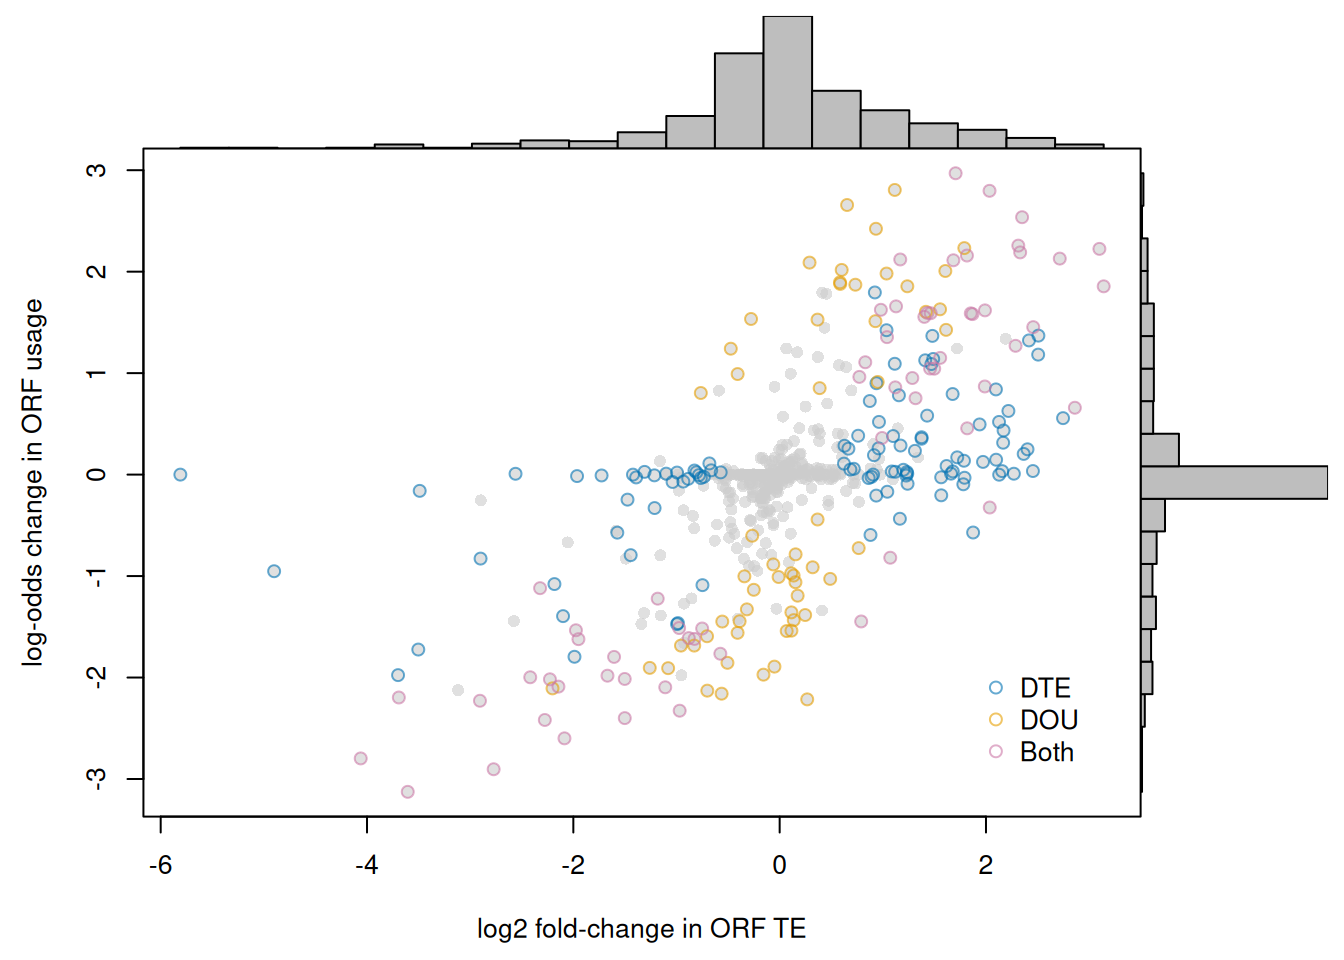
\includegraphics[keepaspectratio]{DOTSeq_files/figure-latex/plotdot-1.png}}
\pandocbounded{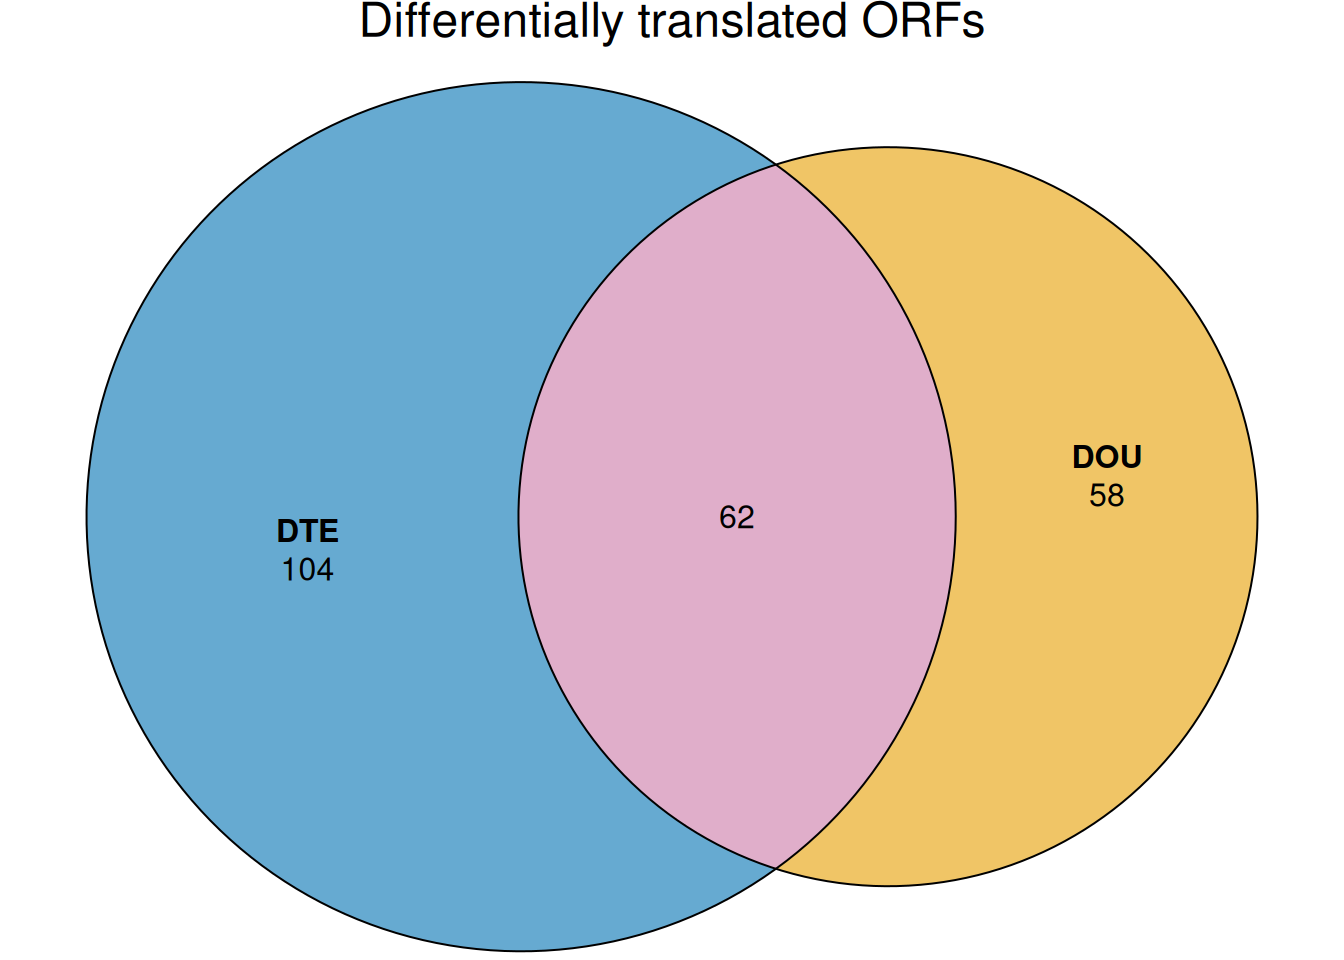
\includegraphics[keepaspectratio]{DOTSeq_files/figure-latex/plotdot-2.png}}

Users can also specify which ORF they want to compare on the heatmap and
it will be saved as a .pdf format. For example, this heatmap is showing
the differential translation between uORF and mORF:

\begin{Shaded}
\begin{Highlighting}[]
\NormalTok{dou\_go }\OtherTok{\textless{}{-}} \FunctionTok{plotHeatmap}\NormalTok{(}\AttributeTok{results =}\NormalTok{  df, }\AttributeTok{orf\_type =} \StringTok{"uORF"}\NormalTok{, }\AttributeTok{flip\_sign =} \ConstantTok{TRUE}\NormalTok{, }\AttributeTok{species\_dataset =} \StringTok{"hsapiens\_gene\_ensembl"}\NormalTok{, }\AttributeTok{symbol\_col =} \StringTok{"hgnc\_symbol"}\NormalTok{)}
\end{Highlighting}
\end{Shaded}

\pandocbounded{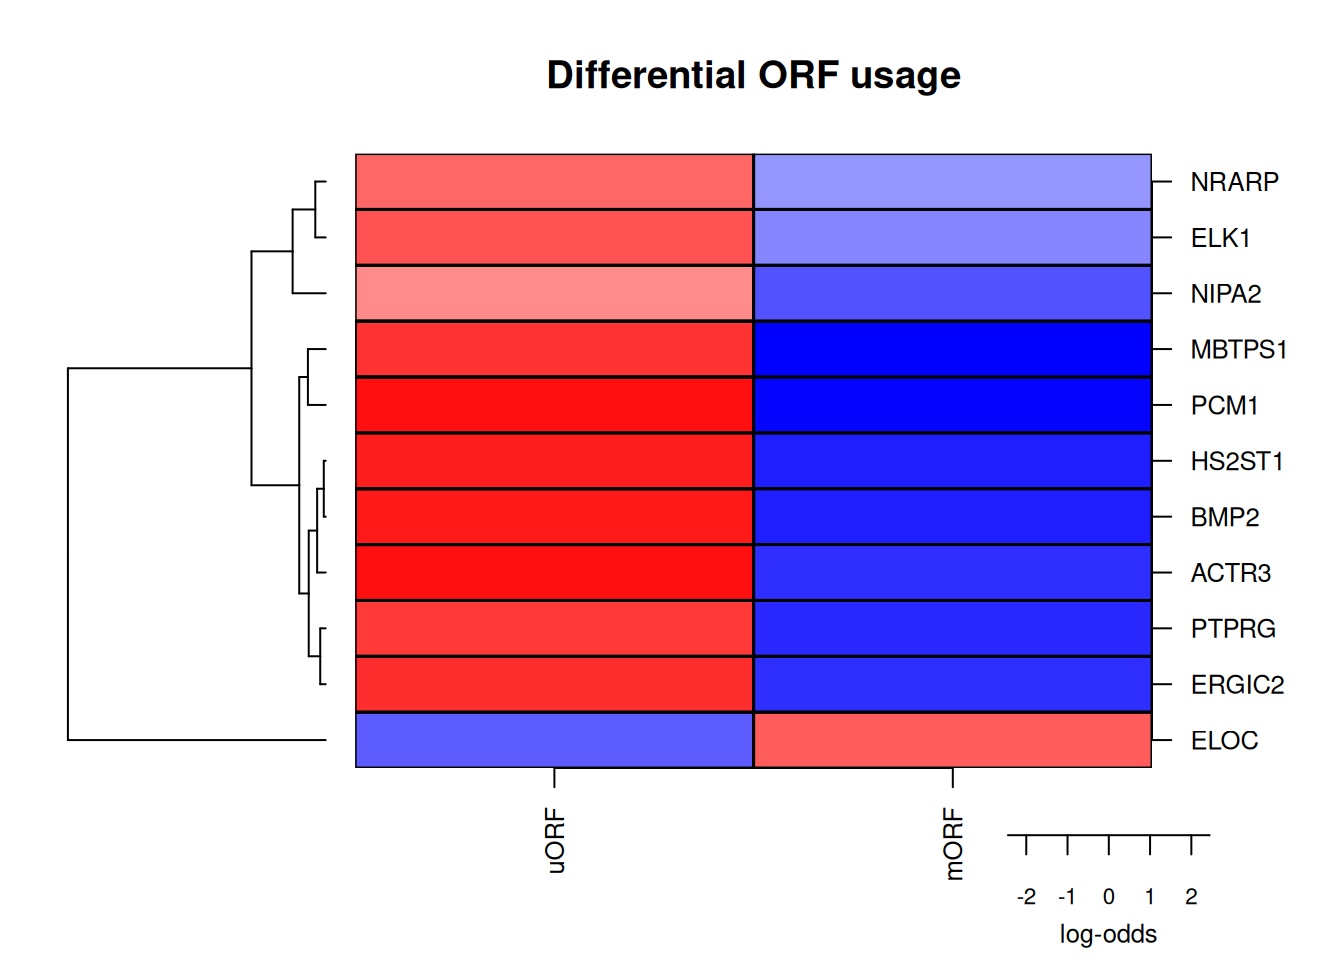
\includegraphics[keepaspectratio]{DOTSeq_files/figure-latex/uORF_heatmap-1.png}}

\section{Session Info}\label{session-info}

\begin{Shaded}
\begin{Highlighting}[]
\FunctionTok{sessionInfo}\NormalTok{()}
\end{Highlighting}
\end{Shaded}

\begin{verbatim}
## R version 4.5.0 (2025-04-11)
## Platform: x86_64-pc-linux-gnu
## Running under: Ubuntu 24.04.2 LTS
## 
## Matrix products: default
## BLAS:   /usr/lib/x86_64-linux-gnu/openblas-pthread/libblas.so.3 
## LAPACK: /usr/lib/x86_64-linux-gnu/openblas-pthread/libopenblasp-r0.3.26.so;  LAPACK version 3.12.0
## 
## locale:
##  [1] LC_CTYPE=en_US.UTF-8       LC_NUMERIC=C               LC_TIME=en_US.UTF-8        LC_COLLATE=en_US.UTF-8    
##  [5] LC_MONETARY=en_US.UTF-8    LC_MESSAGES=en_US.UTF-8    LC_PAPER=en_US.UTF-8       LC_NAME=C                 
##  [9] LC_ADDRESS=C               LC_TELEPHONE=C             LC_MEASUREMENT=en_US.UTF-8 LC_IDENTIFICATION=C       
## 
## time zone: Etc/UTC
## tzcode source: system (glibc)
## 
## attached base packages:
## [1] stats4    stats     graphics  grDevices utils     datasets  methods   base     
## 
## other attached packages:
##  [1] DOTSeq_0.26                 locfdr_1.1-8                satuRn_1.17.0              
##  [4] emmeans_1.11.2-8            ashr_2.2-63                 glmmTMB_1.1.12             
##  [7] DEXSeq_1.55.1               RColorBrewer_1.1-3          AnnotationDbi_1.71.1       
## [10] DESeq2_1.49.4               BiocParallel_1.43.4         SummarizedExperiment_1.39.1
## [13] Biobase_2.69.0              MatrixGenerics_1.21.0       matrixStats_1.5.0          
## [16] rtracklayer_1.69.1          GenomicRanges_1.61.1        Seqinfo_0.99.2             
## [19] IRanges_2.43.0              S4Vectors_0.47.0            BiocGenerics_0.55.1        
## [22] generics_0.1.4              biomaRt_2.65.1              rmarkdown_2.29             
## [25] knitr_1.50                 
## 
## loaded via a namespace (and not attached):
##   [1] splines_4.5.0            later_1.4.2              BiocIO_1.19.0            bitops_1.0-9            
##   [5] filelock_1.0.3           tibble_3.3.0             polyclip_1.10-7          XML_3.99-0.18           
##   [9] lifecycle_1.0.4          httr2_1.2.1              Rdpack_2.6.4             mixsqp_0.3-54           
##  [13] rprojroot_2.1.0          lattice_0.22-7           MASS_7.3-65              magrittr_2.0.3          
##  [17] limma_3.65.3             sass_0.4.10              jquerylib_0.1.4          yaml_2.3.10             
##  [21] remotes_2.5.0            httpuv_1.6.16            sessioninfo_1.2.3        pkgbuild_1.4.8          
##  [25] pbapply_1.7-4            DBI_1.2.3                minqa_1.2.8              eulerr_7.0.2            
##  [29] DHARMa_0.4.7             abind_1.4-8              pkgload_1.4.0            purrr_1.1.0             
##  [33] RCurl_1.98-1.17          rappdirs_0.3.3           sandwich_3.1-1           irlba_2.3.5.1           
##  [37] testthat_3.2.3           genefilter_1.91.0        annotate_1.87.0          commonmark_2.0.0        
##  [41] codetools_0.2-20         DelayedArray_0.35.2      xml2_1.3.8               tidyselect_1.2.1        
##  [45] farver_2.1.2             lme4_1.1-37              BiocFileCache_2.99.5     roxygen2_7.3.2          
##  [49] GenomicAlignments_1.45.2 jsonlite_2.0.0           ellipsis_0.3.2           survival_3.8-3          
##  [53] polylabelr_0.3.0         bbmle_1.0.25.1           tools_4.5.0              progress_1.2.3          
##  [57] Rcpp_1.1.0               glue_1.8.0               SparseArray_1.9.1        xfun_0.52               
##  [61] mgcv_1.9-3               usethis_3.1.0            polyester_1.29.1         dplyr_1.1.4             
##  [65] withr_3.0.2              numDeriv_2016.8-1.1      fastmap_1.2.0            boot_1.3-31             
##  [69] digest_0.6.37            truncnorm_1.0-9          R6_2.6.1                 mime_0.13               
##  [73] estimability_1.5.1       RSQLite_2.4.2            prettyunits_1.2.0        httr_1.4.7              
##  [77] htmlwidgets_1.6.4        S4Arrays_1.9.1           pkgconfig_2.0.3          gtable_0.3.6            
##  [81] rsconnect_1.5.0          blob_1.2.4               hwriter_1.3.2.1          XVector_0.49.0          
##  [85] brio_1.1.5               htmltools_0.5.8.1        profvis_0.4.0            geneplotter_1.87.0      
##  [89] TMB_1.9.17               scales_1.4.0             png_0.1-8                reformulas_0.4.1        
##  [93] rstudioapi_0.17.1        logspline_2.1.22         rjson_0.2.23             coda_0.19-4.1           
##  [97] nlme_3.1-168             curl_7.0.0               nloptr_2.2.1             bdsmatrix_1.3-7         
## [101] cachem_1.1.0             zoo_1.8-14               stringr_1.5.1            parallel_4.5.0          
## [105] miniUI_0.1.2             restfulr_0.0.16          desc_1.4.3               apeglm_1.31.0           
## [109] pillar_1.11.0            grid_4.5.0               vctrs_0.6.5              urlchecker_1.0.1        
## [113] promises_1.3.3           dbplyr_2.5.0             xtable_1.8-4             evaluate_1.0.4          
## [117] magick_2.8.7             tinytex_0.57             invgamma_1.2             mvtnorm_1.3-3           
## [121] cli_3.6.5                locfit_1.5-9.12          compiler_4.5.0           Rsamtools_2.25.2        
## [125] rlang_1.1.6              crayon_1.5.3             SQUAREM_2021.1           emdbook_1.3.14          
## [129] plyr_1.8.9               fs_1.6.6                 stringi_1.8.7            Biostrings_2.77.2       
## [133] devtools_2.4.5           Matrix_1.7-3             hms_1.1.3                bit64_4.6.0-1           
## [137] ggplot2_3.5.2            KEGGREST_1.49.1          statmod_1.5.0            shiny_1.11.1            
## [141] rbibutils_2.3            memoise_2.0.1            bslib_0.9.0              bit_4.6.0
\end{verbatim}

\protect\phantomsection\label{refs}
\begin{CSLReferences}{1}{0}
\bibitem[\citeproctext]{ref-Ly2024}
Ly, Jimmy, KeHui Xiang, Kuan-Chung Su, Gunter B. Sissoko, David P.
Bartel, and Iain M. Cheeseman. 2024. {``{Nuclear release of eIF1
restricts start-codon selection during mitosis}.''} \emph{Nature} 635:
490--98. \url{https://doi.org/10.1038/s41586-024-08088-3}.

\end{CSLReferences}

\end{document}
